
%(BEGIN_QUESTION)
% Copyright 2012, Tony R. Kuphaldt, released under the Creative Commons Attribution License (v 1.0)
% This means you may do almost anything with this work of mine, so long as you give me proper credit

Calculate a realistic $C_v$ value for LV-12, given only the information shown on the following P\&ID:

$$\includegraphics[width=15.5cm]{i0007rx01.eps}$$

Also, calculate the approximate pipe size of control valve necessary to achieve this flow capacity, assuming the use of a double-ported globe valve with a contoured plug ($C_d$ = 13).

\vskip 20pt \vbox{\hrule \hbox{\strut \vrule{} {\bf Suggestions for Socratic discussion} \vrule} \hrule}

\begin{itemize}
\item{} A problem-solving technique useful for getting started is to document all relevant information given to you.  What bits of information are found in this given problem that might be relevant to the answer?  Is the given information quite certain, or are there any ambiguities?  Is there any necessary information missing from the problem -- if so, what?
\item{} Identify any assumptions you were forced to make in calculating this control valve's $C_v$ rating.  Then, identify how these assumptions would skew the necessary $C_v$ rating if they were incorrect.
\item{} Identify the principal advantage that a {\it double-ported} globe valve enjoys over a {\it single-ported} globe valve.
\item{} Identify the equivalent cage-guided globe valve type (balanced or unbalanced) to a double-ported stem-guided globe valve.
\end{itemize}

\underbar{file i03216}
%(END_QUESTION)





%(BEGIN_ANSWER)

There is too much uncertainty in the given information to calculate a sure $C_v$ value.  An extremely uncertain answer, though, is $C_v$ = 1.033. 

%(END_ANSWER)





%(BEGIN_NOTES)

Calculating flow capacity ($C_v$) of control valve:

$$Q = C_v \sqrt{\Delta P \over G_f}$$

$$C_v = {Q \over \sqrt{\Delta P \over G_f}}$$

If we use pump P-103 specifications (8 GPM max ; 60 PSI head max), we get:

$$C_v = {8 \over \sqrt{60 \over 1}} = 1.033$$

This is approximate for several reasons.  First, the maximum desired flow for this control valve might not be the maximum flow capacity of P-103 -- it's probably less.  This suggests the real $C_v$ might be lower.  Another factor is that we do not know the pressure drop across the valve at full-open, but it is probably a lot less than than pump's maximum head of 60 PSI.  This suggests the real $C_v$ might be higher.  Finally, the stripped water may very well be hotter than 60 degrees Fahrenheit, which would decrease its density and decrease the necessary $C_v$.

\vskip 10pt

Calculating pipe size of control valve:

$$C_d = {C_v \over d^2}$$

$$d^2 = {C_v \over C_d}$$

$$d = \sqrt{C_v \over C_d}$$

$$d = \sqrt{1.033 \over 13} = 0.282 \hbox{ inches}$$

Rounding up 0.282 inches to the nearest standard pipe size gives 0.375 ($3 \over 8$) or 0.5 ($1 \over 2$) inch nominal.

%INDEX% Final Control Elements, valve: sizing
%INDEX% Process: sour water stripping tower (realistic P&ID shown)

%(END_NOTES)


